\documentclass[20pt]{article}
\usepackage[T2A]{fontenc}
\usepackage{mathtools}
\usepackage[utf8]{inputenc}
\usepackage[english, russian]{babel}
\usepackage{gensymb}
\usepackage{floatrow}
\usepackage{fancyhdr}

\pagestyle{fancy}
\author{}
\title{Определение теплоты испарения жидкости}
\lhead{Работа 2.4.1}
\rhead{Терехов Максим 876}
\date{}

\begin{document}
\selectlanguage{russian}
\parindent=1cm
\large
\maketitle
\section{Цель работы:}
1) измерение давления насыщенного пара жидкости при разной температуре;
2) вычисление по полученным данным теплоты испарения с помощью уравнения Клапейрона–Клаузиуса.
\section{В работе используются:}
термостат; герметический сосуд, заполненный исследуемой жидкостью; отсчетный микроскоп.
\section{Экспериментальная установка:}
\begin{figure}[H]\begin{figure}[H]
\center
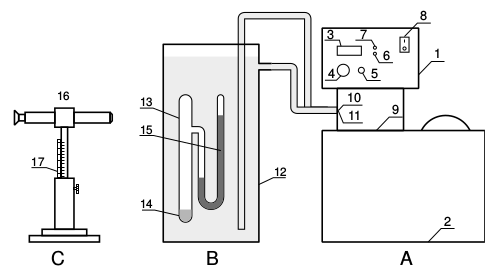
\includegraphics[scale=0.5]{asd.png}
\end{figure}
\center
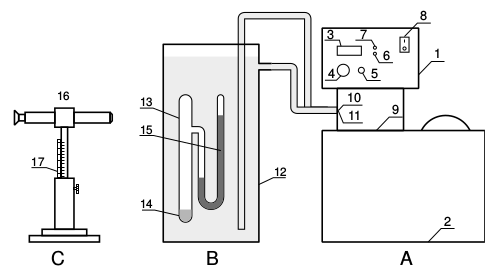
\includegraphics[scale=0.5]{asd.png}
\end{figure}
\section{Теоретическая часть:}
Испарением называется переход вещества из жидкого в газообразное состояние. 
Оно происходит на свободной поверхности жидкости. При испарении с поверхности 
вылетают молекулы, образуя над ней пар. Для выхода из жидкости молекулы должны 
преодолеть силы молекулярного сцепления. Кроме того, при испарении совершается 
работа против внешнего давления $P$ , поскольку объем жидкости меньше объема 
пара. Не все молекулы жидкости способны совершить эту работу, а только те из 
них, которые обладают достаточной кинетической энергией. Поэтому переход части 
молекул в пар приводит к обеднению жидкости быстрыми молекулами, т. е. к ее 
охлаждению. Чтобы испарение проходило без изменения температуры, к жидкости
нужно подводить тепло. Количество теплоты, необходимое для изотермического 
испарения одного моля жидкости при внешнем давлении, равном упругости ее 
насыщенных паров, называется молярной теплотой испарения (парообразования).

Теплоту парообразования жидкостей можно измерить непосредственно при помощи 
калориметра. Такой метод, однако, не позволяет получить точных результатов из-
за неконтролируемых потерь тепла, которые трудно сделать малыми. В настоящей 
работе для определения теплоты испарения применен косвенный метод, основанный 
на формуле Клапейрона–Клаузиуса:
\begin{equation}
	\frac{dP}{dT} = \frac{L}{T(V_2-V_1)}.
\end{equation}
Здесь $P$ --- давление насыщенного пара жидкости при температуре
$T$ , $T$ --- абсолютная температура жидкости и пара, $L$ --- теплота испарения жидкости, $V_2$ --- объем пара, $V_1$ --- объем жидкости. Найдя из
опыта $dP/dT$, $T$, $V_2$ и $V_1$, можно определить $L$ путем расчета. Вели-
чины $L$, $V_2$ и $V_1$ в формуле  должны относиться к одному и тому
же количеству вещества; мы будем относить их к одному молю.

В нашем приборе измерения производятся при давлениях ниже
атмосферного. В этом случае задача существенно упрощается.

В таблице для ряда жидкостей приведены: температура, при которой давление насыщенных паров равно атмосферному, величины $V_2$ и $V_1$, входящие в (1), а также константы a и b в уравнении Ван-дер-Ваальса.

\noindent
\begin{tabular}{|c|c|c|c|c|c|c|}
\hline Вещество &  $T_{\text{кип}}$ & $V_1,$ & $V_2,$ & $b$ & $a$ & $a/{V_2}^2$ \\
 &  & $10^{-6}$ & $10^{-3}$ & $10^{-6}$ & & \\
 & K & $\frac{\text{м}^3}{\text{моль}}$ & $\frac{\text{м}^3}{\text{моль}}$ &
 $\frac{\text{м}^3}{\text{моль}}$ & $\frac{\text{Па} \cdot \text{м}^6}{\text{моль}^2}$ & кПа \\
\hline Вода & $373$ & $18$ & $31$ & $26$ & $0.4$ & $0.42$ \\
$CCl_4$ & $350$ & $97$ & $29$ & $126$ & $1.95$ & $2.3$ \\
Этиловый эфир & $307$ & $104$ & $25$ & $137$ & $1.8$ & $2.9$ \\
Этиловый спирт & $351$ & $58$ & $29$ & $84$ & $1.2$ & $1.4$ \\
\hline
\end{tabular}


Из таблицы видно, что $V_1$ не превосходит 0,5\% от $V_2$. При нашей
точности опытов величиной $V_1$ в (1) можно пренебречь.

Обратимся теперь к $V_2$, которое в дальнейшем будем обозначать
просто $V$. Объем $V$ связан с давлением и температурой уравнением
Ван-дер-Ваальса:
\[
	\left( P + \frac{a}{V^2} \right) \left( V - b \right) = RT.
\]
Из рассмотрения таблицы следует, что $b$ одного порядка с $V_1$. В уравнении Ван-дер-Ваальса величиной $b$ следует пренебречь. Пренебреже-
ние членом $a/V^2$ по сравнению с $P$ вносит ошибку менее 3\%. При давлении ниже атмосферного ошибки становятся еще меньше. Таким образом, при давлениях ниже атмосферного уравнение Ван-дер-Ваальса для насыщенного пара мало отличается от уравнения Клапейрона.
Положим поэтому
\begin{equation}
	V = \frac{RT}{P}.
\end{equation}
Подставляя (2) в (1), пренебрегая $V_1$ и разрешая уравнение относительно
$L$, найдем
\[
	L = \frac{RT^2}{P} \frac{dP}{dT} = -R \frac{d(\ln P)}{d(1/T)}.
\]
Эта формула является окончательной.

В нашем опыте температура жидкости измеряется термометром, давление пара определяется при помощи манометра, а производные $dP/dT$ или $d(\ln P)/d(1/T)$ находятся графически как угловой коэффициент касательной к кривой $P(T)$ или соответственно к кривой, у которой по оси абсцисс отложено $1/T$, а по оси ординат $\ln P$.
\section{Обработка результатов измерений:}
Исследуемая жидкость --- вода.
Давление пара находится по следующей формуле:
\[
	P = \rho g \Delta h,
\]
где $\rho$ --- плотность ртути, $\Delta h = h_1 - h_2$ --- разница высот в ртуртном манометре.
\begin{figure}[H]
	\begin{floatrow}
		\ttabbox{\caption{Нагревание}}{
				\begin{tabular}{|c|c|c|c|c|}
					\hline $T, K$ & $H_1, \text{мм}$ & $H_2, \text{мм}$ & $\Delta h, \text{мм}$ & $P, \text{Па}$
					 \\\hline $298$ & $94.25$ & $71.35$ & $22.90$ & $3043.10$
					 \\\hline $299$ & $94.90$ & $70.50$ & $24.40$ & $3242.42$
					 \\\hline $300$ & $95.70$ & $70.00$ & $25.70$ & $3415.18$
					 \\\hline $301$ & $96.50$ & $69.20$ & $27.30$ & $3627.79$
					 \\\hline $302$ & $97.30$ & $68.50$ & $28.80$ & $3827.12$
					 \\\hline $303$ & $98.20$ & $67.70$ & $30.50$ & $4053.03$
					 \\\hline $304$ & $99.15$ & $66.85$ & $32.30$ & $4292.23$
					 \\\hline $305$ & $100.00$ & $65.80$ & $34.20$ & $4544.71$
					 \\\hline $306$ & $101.50$ & $64.95$ & $36.55$ & $4856.99$
					 \\\hline $307$ & $102.20$ & $63.75$ & $38.45$ & $5109.48$
					 \\\hline $308$ & $103.30$ & $62.95$ & $40.35$ & $5361.96$
					 \\\hline $309$ & $104.40$ & $61.60$ & $42.80$ & $5687.53$
					 \\\hline $310$ & $105.80$ & $60.50$ & $45.30$ & $6019.75$
					 \\\hline $311$ & $107.20$ & $59.25$ & $47.95$ & $6371.90$
					 \\\hline $312$ & $108.30$ & $57.80$ & $50.50$ & $6710.76$
					 \\\hline $313$ & $109.90$ & $56.60$ & $53.30$ & $7082.84$\\\hline
				\end{tabular}}
		\ttabbox{\caption{Охлаждение}}{
				\begin{tabular}{|c|c|c|c|c|}
					\hline $T, K$ & $H_1, \text{мм}$ & $H_2, \text{мм}$ & $\Delta h, \text{мм}$ & $P, \text{Па}$
					 \\\hline $298$ & $94.40$ & $71.10$ & $23.30$ & $3096.25$
					 \\\hline $299$ & $95.15$ & $70.50$ & $24.65$ & $3275.65$
					 \\\hline $300$ & $95.90$ & $70.00$ & $25.90$ & $3441.75$
					 \\\hline $301$ & $96.80$ & $69.00$ & $27.80$ & $3694.24$
					 \\\hline $302$ & $97.60$ & $68.15$ & $29.45$ & $3913.50$
					 \\\hline $303$ & $98.55$ & $67.20$ & $31.35$ & $4165.98$
					 \\\hline $304$ & $99.40$ & $66.65$ & $32.75$ & $4352.03$
					 \\\hline $305$ & $100.75$ & $65.40$ & $35.35$ & $4697.53$
					 \\\hline $306$ & $101.50$ & $64.50$ & $37.00$ & $4916.79$
					 \\\hline $307$ & $102.60$ & $63.10$ & $39.50$ & $5249.01$
					 \\\hline $308$ & $103.60$ & $62.55$ & $41.05$ & $5454.98$
					 \\\hline $309$ & $104.80$ & $61.40$ & $43.40$ & $5767.26$
					 \\\hline $310$ & $106.10$ & $60.20$ & $45.90$ & $6099.48$
					 \\\hline $311$ & $107.60$ & $59.00$ & $48.60$ & $6458.27$
					 \\\hline $312$ & $108.80$ & $57.50$ & $51.30$ & $6817.07$
					 \\\hline $313$ & $109.90$ & $56.60$	& $53.30$ & $7082.84$\\\hline
		\end{tabular}
		}
	\end{floatrow}
\end{figure}
Построим графики в координатах $T, P$ и в координатах $1/T, \ln P$ и найдем угловой коэффициент по методу наименьших квадратов:
\begin{figure}[H]
	\caption{График в координатах $T, P$}
	\center
	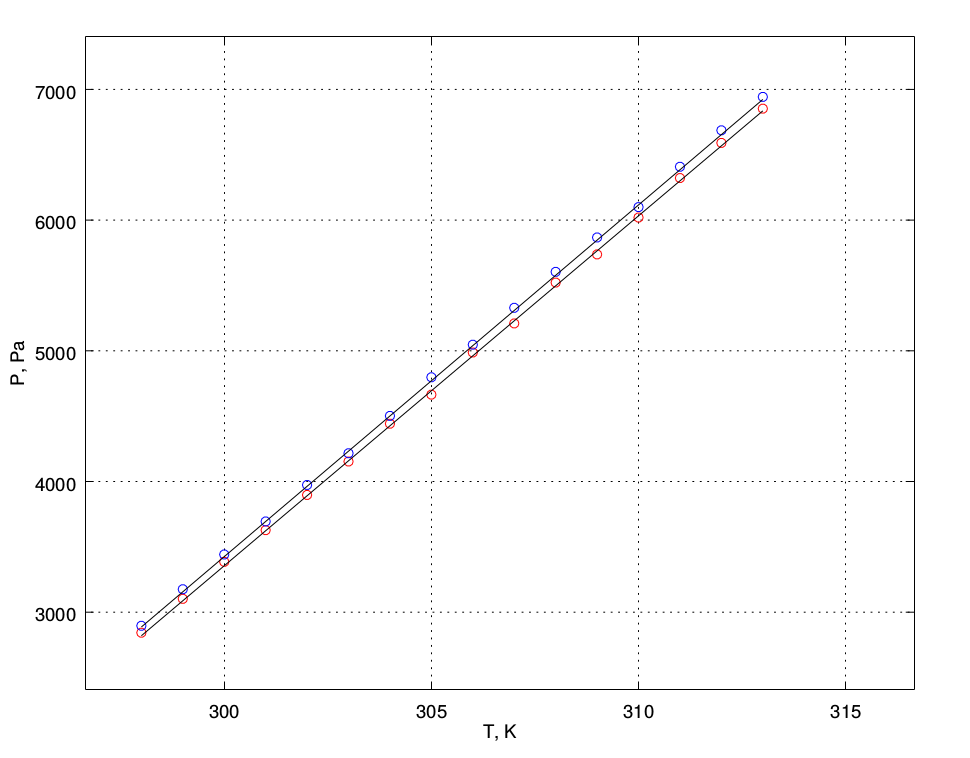
\includegraphics[scale=0.3]{PT.png}
\end{figure}
Угловые коэффициенты графика в координатах $T, P$:

 $a_{\text{наг}_1} = 267.75$; $a_{\text{охл}_1} = 269.11$.
 \begin{figure}[H]
	\caption{График в координатах $1/T, \ln P$}
	\center
	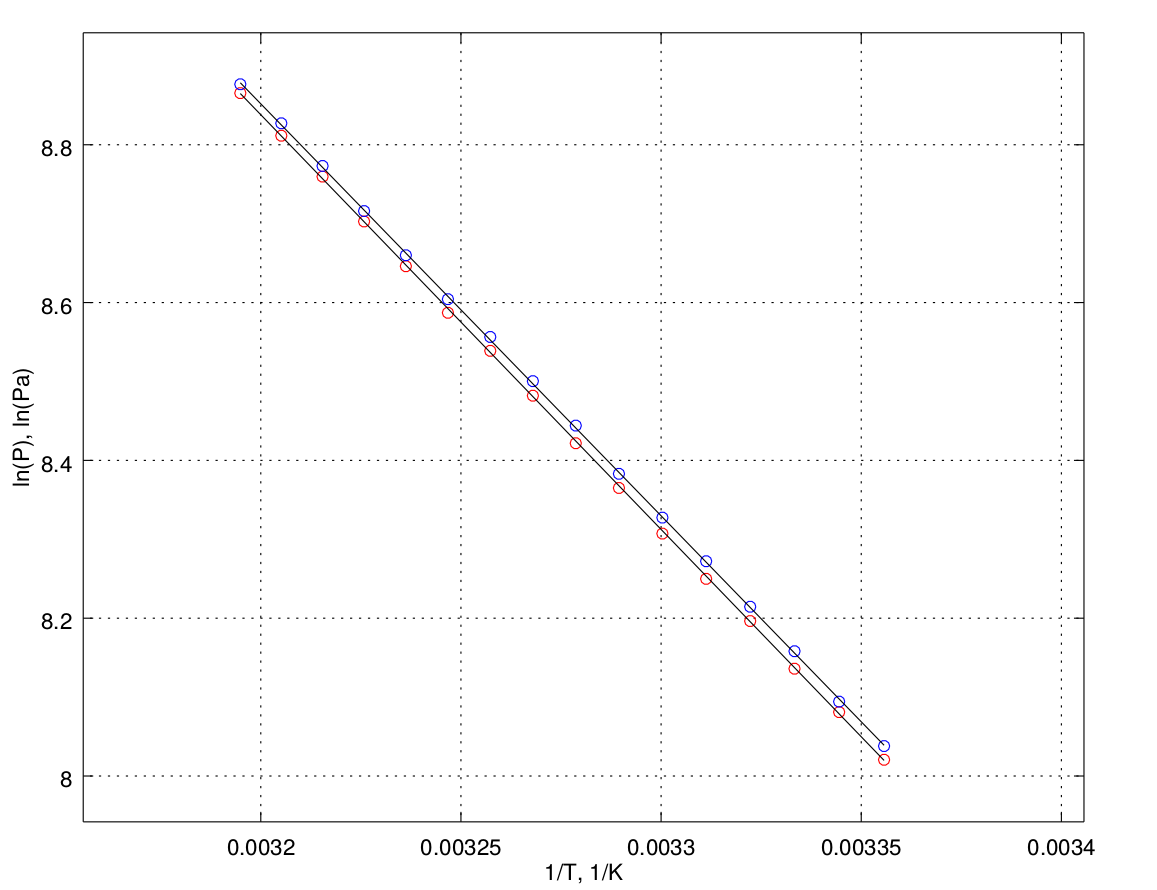
\includegraphics[scale=0.3]{ln.png}
\end{figure}
Угловые коэффициенты графика в координатах $1/T, \ln P$:

 $a_{\text{наг}_2} = -\textsc{5255.273}$, $a_{\text{охл}_2} = -5240.746$.
 Оценим погрешности: 
\[
\varepsilon_{h_1} = \varepsilon_{h_1} = 0.0122 = 1.22\%
\]
\[
 \varepsilon_P = \sqrt{\varepsilon_{h_1}^2 + \varepsilon_{h_2}^2} = 0.0173 = 1.73\%
\]
\[
\varepsilon_T = 0.0003 = 0.03\%
\]
\[
\varepsilon_L = \sqrt{\varepsilon_T^2 + \varepsilon_P^2} = 0.0174 = 1.74\%
\]
 Рассчитаем теплоту испарения жидкости по формуле:
 \[
 	L = \frac{RT}{P} \frac{dP}{dT} = -R \frac{d(\ln P)}{d(1/T)}.
 \]
 \[
L_{\text{наг}_1} = 37897.82\ \text{Дж} = 37.9\ \text{кДж}
\]
 \[
L_{\text{охл}_1} = 39039.53\ \text{Дж} = 39.0\ \text{кДж}
\]
\[
L_{\text{наг}_2} = 40671.31\ \text{Дж} = 40.7\ \text{кДж}
\]
 \[
L_{\text{охл}_2} = 40550.59\ \text{Дж} = 40.6\ \text{кДж}
\]
Результат косвенного вычисления $L$ по коэффициенту наклона прямой более точен во втором случае, так как в конечную формулу входит меньше измеряемых физических величин, а следовательно и погрешность меньше.
\[
L_{\text{наг}} = 40.7\pm 0.74\ \text{кДж}
\]
 \[
L_{\text{охл}} = 40.6\pm 0.73\ \text{кДж}
\]
Таблбичное значение теплоты испарения воды для 1 моля:
\[
L_{\text{табл}} = 40.2\ \text{кДж}
\]
\end{document}